 \chapter{Numerical Results} \label{Chptr5}

\noindent \noindent \hrulefill

In this chapter we present the numerical results and compare the algorithms presented in this work with other center-based algorithms that are commonly used to address the clustering problem. We describe in detail the setting used in each comparison. We compare the commonly used parameters, such as function objective values and number of iterations until a certain precision is achieved. In addition to these parameters, we use several different types of clustering metrics to compare the final clusterings obtained by the discussed algorithms. 

\noindent \noindent \hrulefill

Most of the existing clustering methods are sensitive to the starting point, namely choosing different starting point result in significant differences in the final clustering. There are plethora of heuristic initialization methods. One such initialization method is to choose $k$ random data points as staring centers, assuming uniform distribution or some other prior distribution on the data. Another popular initialization method is to label at random each data point, assuming uniform distribution over the labels for each point. \medskip

The initialization points used within the implementation of the compared algorithms are as follows. k-means staring point is constructed by randomly choosing $k$ different points from the dataset. The same technique is employed in the cases of KPALM and $\varepsilon$-KPALM, for the $x(0)$ variable. Whereas for the $w(0)$ variable, it is chosen at random from $\Delta^m$. k-means++ takes also part in our comparison, and it is basically the same as k-means, with the exception of its starting point that is constructed in the following manner. The first center $x^1(0)$ is chosen randomly from the dataset $\mathcal{A}$. Suppose that $1 \leq l < k$ centers have already been chosen, set $x^{l+1}(0)$ to be the point in the dataset that is the furthest from its closest center.

Since it is impractical to compare the function values achieved with the algorithms which solve the squared Euclidean clustering problem with that of the algorithms which solve the Euclidean clustering problem, we used some criteria devised to compare clustering partitions. Criteria such as \textit{variation of information (VI)}, \textit{Mirkin metric}, and \textit{Van Dongen metric}, are few examples for metrics that measure the difference between two clustering partitions (see \cite{M2005}). With these metrics we compared the similarity of the partition achieved with each algorithm to the desired partition of each dataset. The goal is to decrease the value of the metrics.

\section{Iris Dataset}
We used the famous Iris dataset to test the performance of the KPALM algorithm. It is important to note that choosing the parameter $\alpha$ is left to the user, and as presented below, has a significant effect on the convergence rate and the quality of the achieved clustering, namely the value of the objective function over the generated series. All the plots in this section are made by averaging over $100$ trials, each trial with random starting point.
\begin{figure}[h]
    \centering
    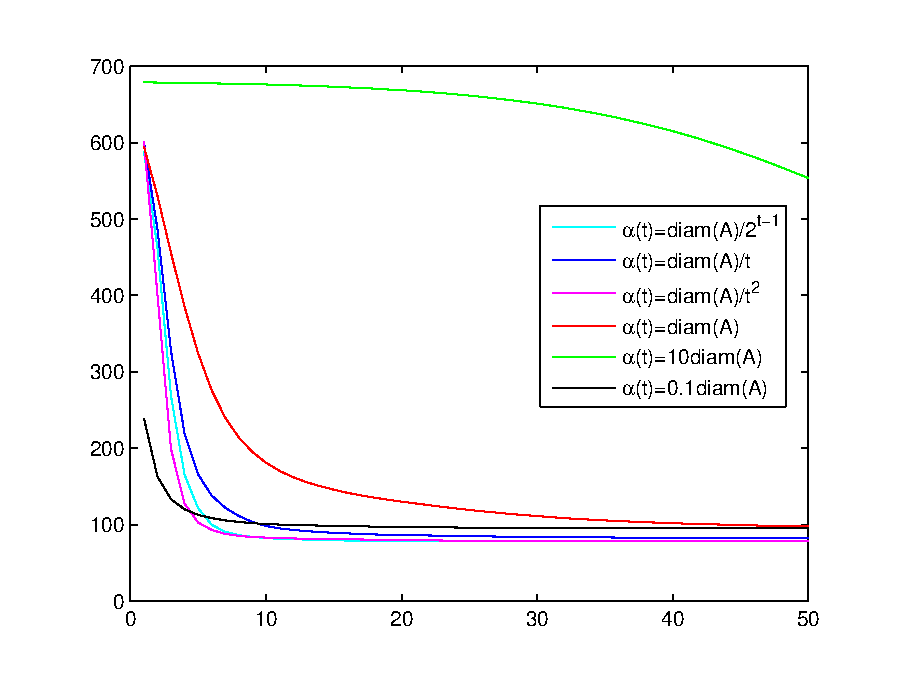
\includegraphics[width=0.8\textwidth]{dynamic_alpha_kpalm}
    \caption{Comparison of the objective values for different values of $\alpha$.}
    \label{fig:dynamic_alpha_psi_comp}
\end{figure} 
\Cref{fig:dynamic_alpha_psi_comp} shows that dynamic values of the parameter $\alpha$ which decreases fast, such as $\alpha_i(t)=
\frac{diam(\mathcal{A})}{2^{t-1}}$, achieve smaller function values. 
Similarly to \Cref{fig:dynamic_alpha_psi_comp}, in \Cref{fig:dynamic_alpha_eps_psi_comp} we can see a comparison of the objective values of $\sigma_{\varepsilon}$ for different function values. The value of $\varepsilon$ is set to be 1e-5.

\noindent In \Cref{fig:algs_psi_comp} we made a comparison between KPALM with dynamic rule for choosing the parameter $\alpha$, that is $\alpha_i(t)=\frac{diam(\mathcal{A})}{2^{t-1}}$, with k-means and k-means++. It demonstrates that KPALM can reach lower objective function values then k-means, and these are similar to the values achieved with KMEAN++. In addition, the KPALM++ are the objective function values achieved with KPALM when the $x$ variable is initialized as in k-means++. Unlike k-means, the objective function values KPALM converge to are more stable and less sensitive to its starting point.
\begin{figure}
    \centering
    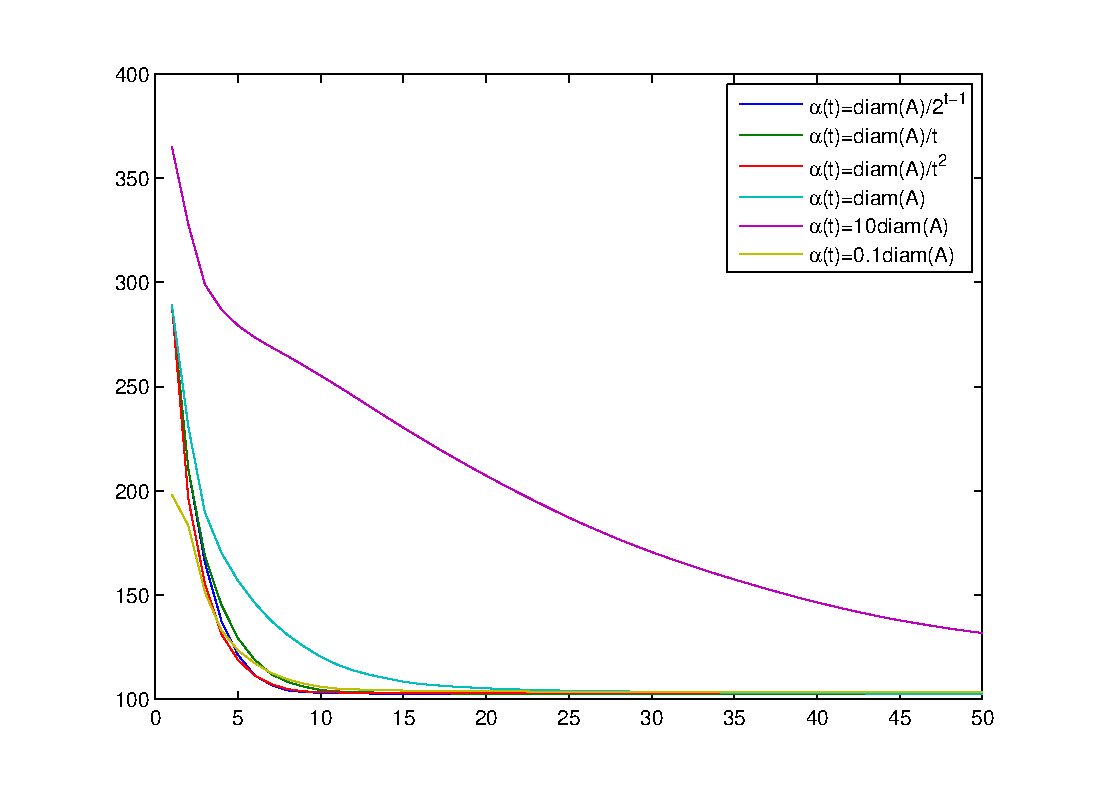
\includegraphics[width=0.75\textwidth]{dynamic_alpha_eps_kpalm}
    \caption{Comparison of the objective values for different values of $\alpha$.}
    \label{fig:dynamic_alpha_eps_psi_comp}
\end{figure}
\begin{figure}[ht]
    \centering
    \begin{subfigure}[b]{0.8\textwidth}
        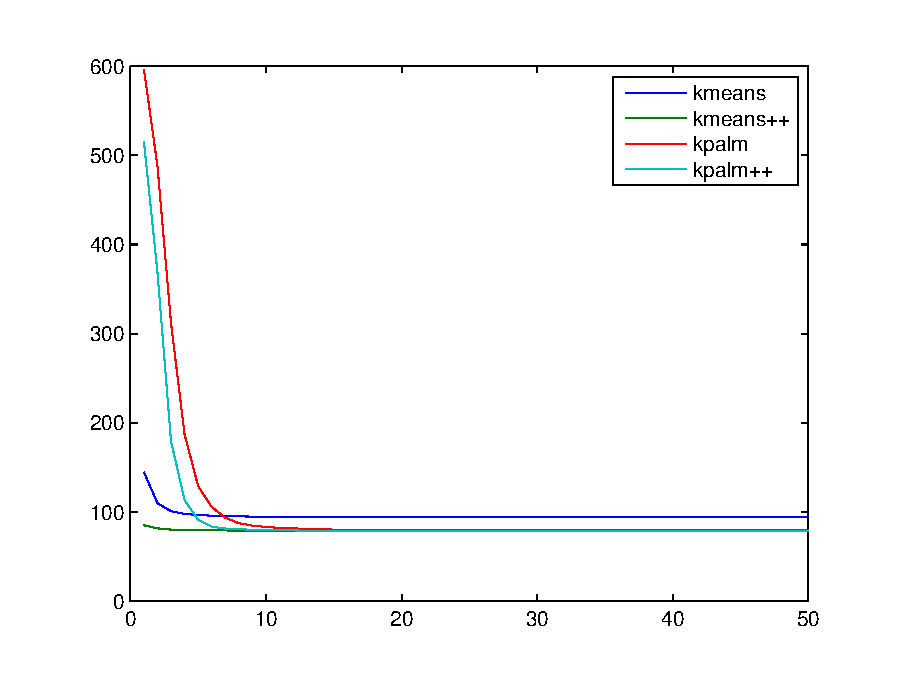
\includegraphics[width=\textwidth]{psi_algs_comparison2}
        \caption{Comparison of objective function values.}
        \label{fig:algs_psi_comp_A}
    \end{subfigure}
    \begin{subfigure}[b]{0.8\textwidth}
        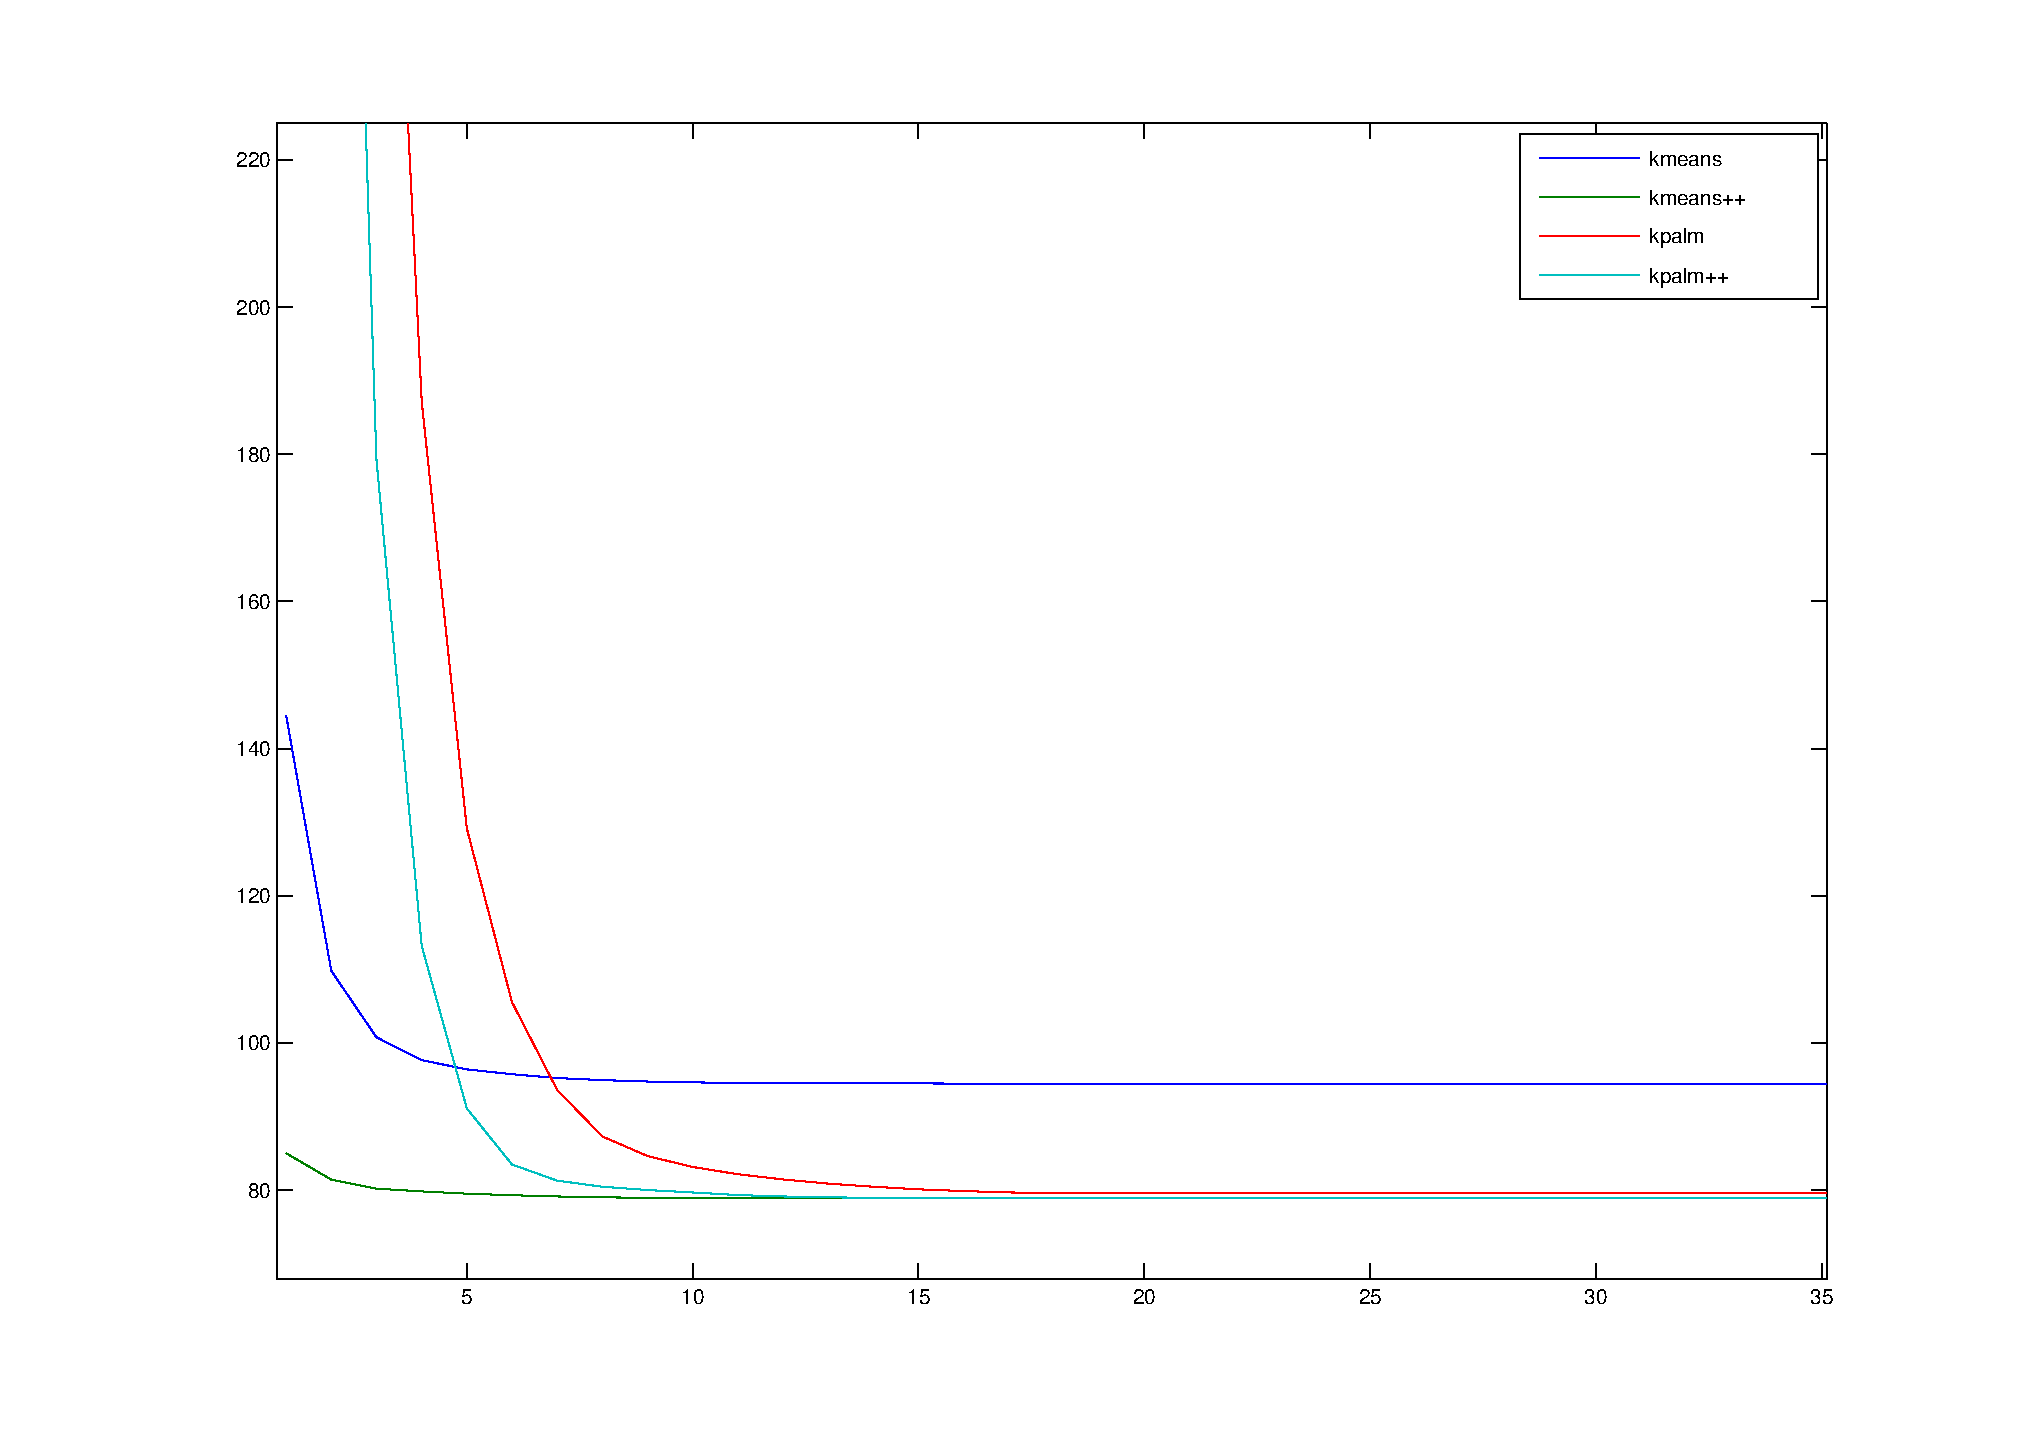
\includegraphics[width=\textwidth]{psi_algs_comparison2_zoom}
        \caption{Zoom of \Cref{fig:algs_psi_comp_A}.}
        \label{fig:algs_psi_comp_B}
    \end{subfigure}
    \caption{Comparison of objective function values for k-means, k-means++, KPALM and KPALM++.} \label{fig:algs_psi_comp}
\end{figure}
\Cref{fig:iters_comp} shows the number of iteration needed to reach precision of 1e-3 between consecutive objective function values.
\begin{figure}
    \centering
    \begin{subfigure}[b]{0.7\textwidth}
        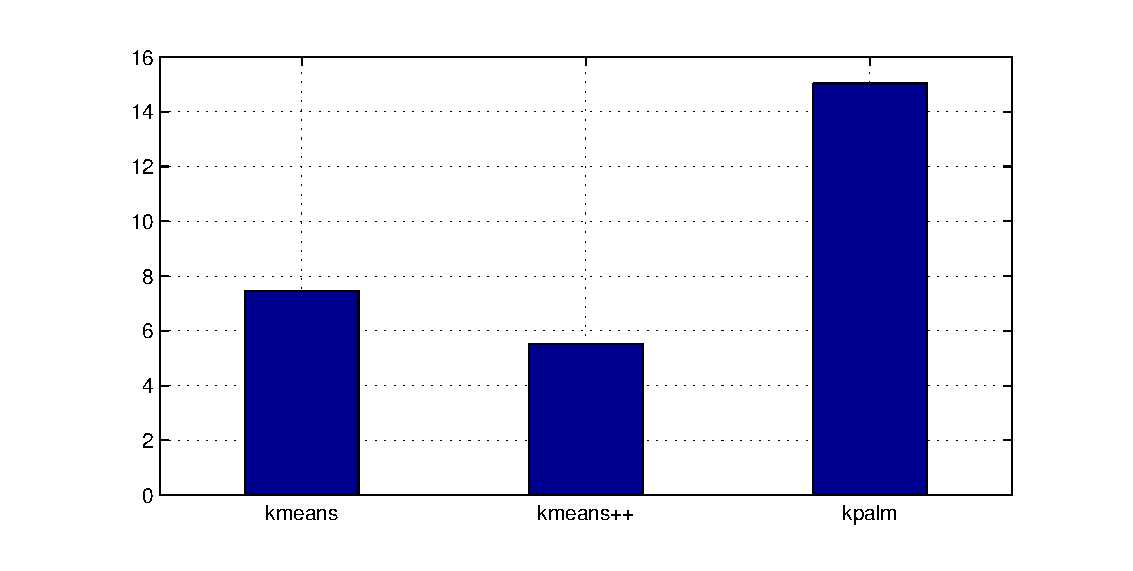
\includegraphics[width=\textwidth]{iterations_algs_comparison}
        \caption{Number of iterations of k-means, k-means++ and KPALM with $\alpha(t)=diam(\mathcal{A})/2^{t-1}$.}
        \label{fig:iters_algs_comp}
    \end{subfigure}
    ~ %add desired spacing between images, e. g. ~, \quad, \qquad, \hfill etc. 
      %(or a blank line to force the subfigure onto a new line)
    \begin{subfigure}[b]{0.7\textwidth}
        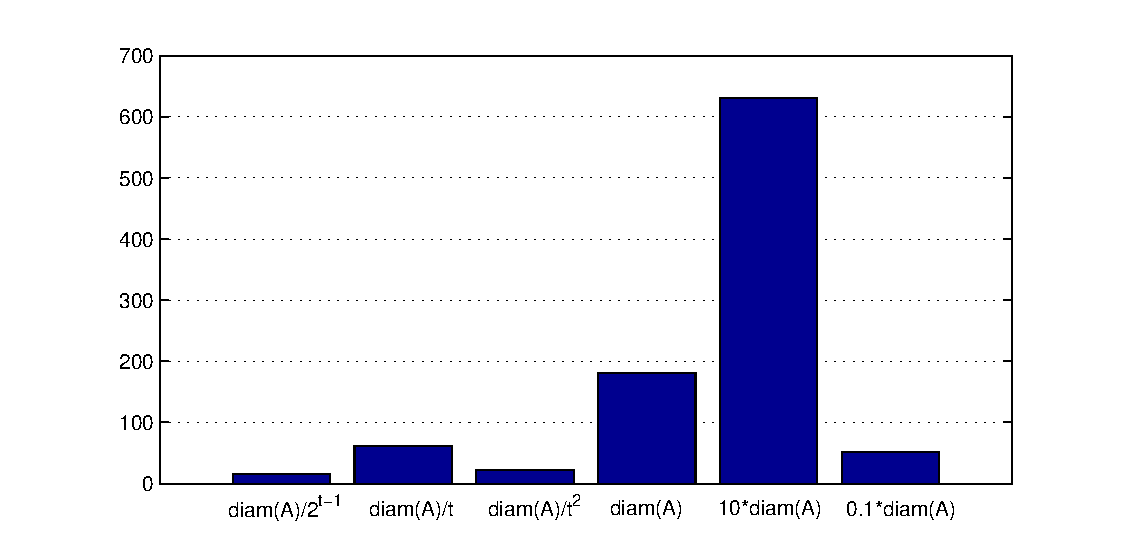
\includegraphics[width=\textwidth]{iterations_dynamic_alpha_kpalm_comparison}
        \caption{Number of iterations of KPALM with different updates of $\alpha(t)$.}
        \label{fig:iters_dyn_alpha_kpalm_comp}
    \end{subfigure}
    \begin{subfigure}[b]{0.7\textwidth}
        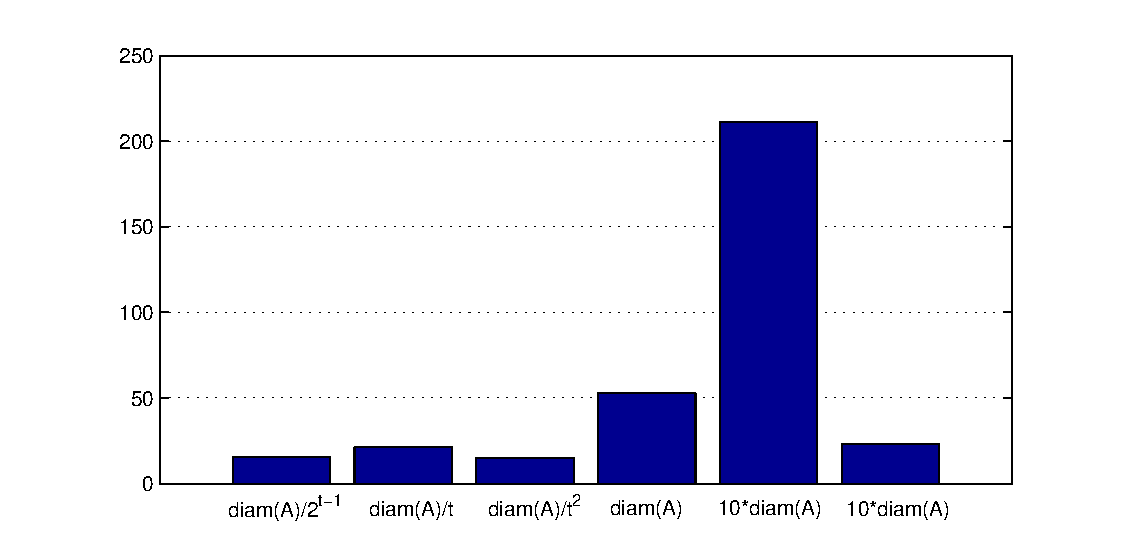
\includegraphics[width=\textwidth]{iterations_dynamic_alpha_eps_kpalm_comparison}
        \caption{Number of iterations of $\varepsilon$-KPALM with different updates of $\alpha(t)$.}
        \label{fig:iters_dyn_alpha_eps_kpalm_comp}
    \end{subfigure}
    \caption{Comparison of number of iterations needed to reach 1e-3 precision of $\sigma$.}\label{fig:iters_comp}
\end{figure}

\FloatBarrier
\section{Synthetic Dataset}
In this section we show that $\varepsilon$-KPALM is less sensitive to outliers in the data verses algorithms that suit the squared Euclidean norm (e.g., k-means, k-means++ and KPALM). We generated two synthetic datasets, each contains 300 points in the plane, by sampling three two-dimensional Gaussian, 100 samples each. In \Cref{fig:gaussians}(\ref{fig:dense_gaussians}) the clusters are denser than in \Cref{fig:gaussians}(\ref{fig:sparse_gaussians}).
Then we run the clustering algorithms and compared their clustering results, namely, how many points were clustered correctly. From \Cref{fig:gaussians_similarity}(\ref{fig:dense_gaussians_similarity}) it is evident that k-means is superior to other algorithms in the dense case and $\varepsilon$-KPALM is quite sensitive. Whereas, in the sparse case in \Cref{fig:gaussians_similarity}(\ref{fig:sparse_gaussians_similarity}), $\varepsilon$-KPALM is superior, and less sensitive to outliers. 
In \Cref{fig:gaussians_metrics} we compare the distance of clusterings achieved with different algorithms to the desired clustering, where kpalm1, kpalm2 and kpalm3 match using $\alpha(t)=diam(\mathcal{A})/2^{t-1}$, $\alpha(t)=diam(\mathcal{A})/t^2$ and $\alpha(t)=diam(\mathcal{A})$ respectively, and similarly for $\varepsilon$-kpalm$i$, $i \in \{1,2,3\}$. 
In \Cref{fig:gaussians_metrics}(\ref{fig:dense_gaussians_metrics}) we witness that for dense dataset, the resulting clusterings of squared Euclidean algorithms, namely, k-means, k-means++ and KPALM, are superior to the clustering $\varepsilon$-KPALM, where KPALM with $\alpha(t)=diam(\mathcal{A})/2^{t-1}$ gives the best result, that is, the clustering in this setting is the closest to the desired clustering. Whereas in the sparse dataset, the clustering achieved with $\varepsilon$-KPALM with $\alpha(t)=diam(\mathcal{A})/t^2$ is the closest to the desired clustering, as reflected from \Cref{fig:gaussians_metrics}(\ref{fig:sparse_gaussians_metrics}).
\begin{figure}[hb]
    \centering
    \begin{subfigure}[b]{0.45\textwidth}
        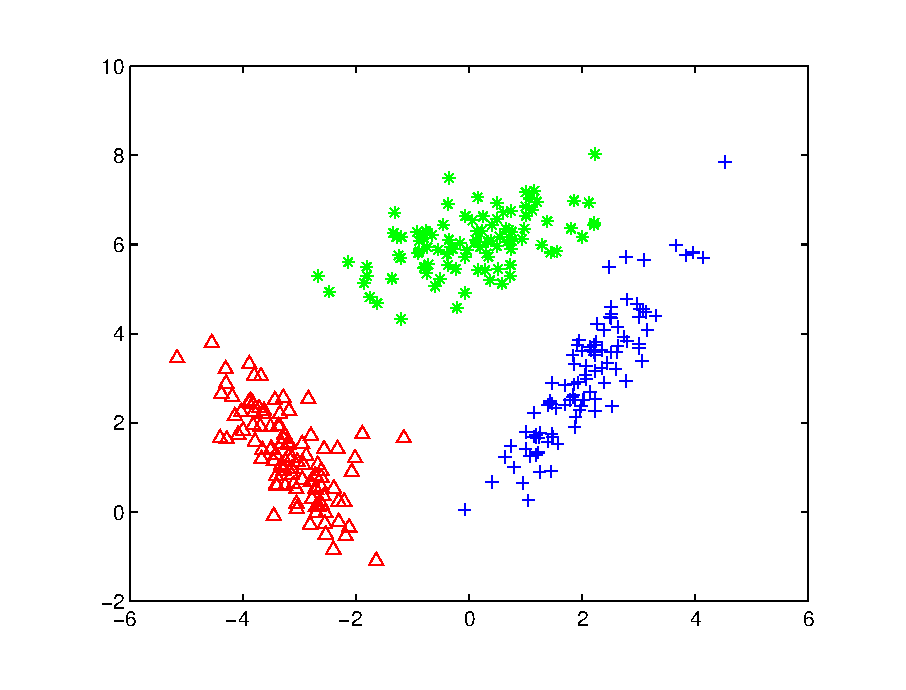
\includegraphics[width=\textwidth]{dense_gaussians}
        \caption{Dense Gaussians.}
        \label{fig:dense_gaussians}
    \end{subfigure}
    \quad
    \begin{subfigure}[b]{0.45\textwidth}
        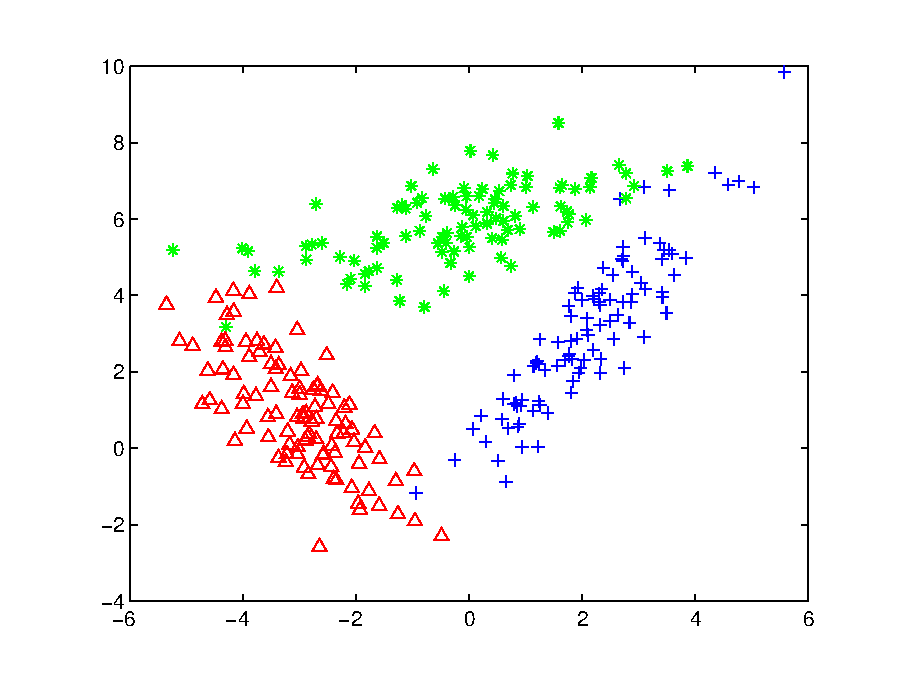
\includegraphics[width=\textwidth]{sparse_gaussians}
        \caption{Sparse Gaussians.}
        \label{fig:sparse_gaussians}
    \end{subfigure}
    \caption{Two datasets, each 300 points.}
    \label{fig:gaussians}
\end{figure}

\begin{figure}
    \centering
    \begin{subfigure}[b]{0.8\textwidth}
        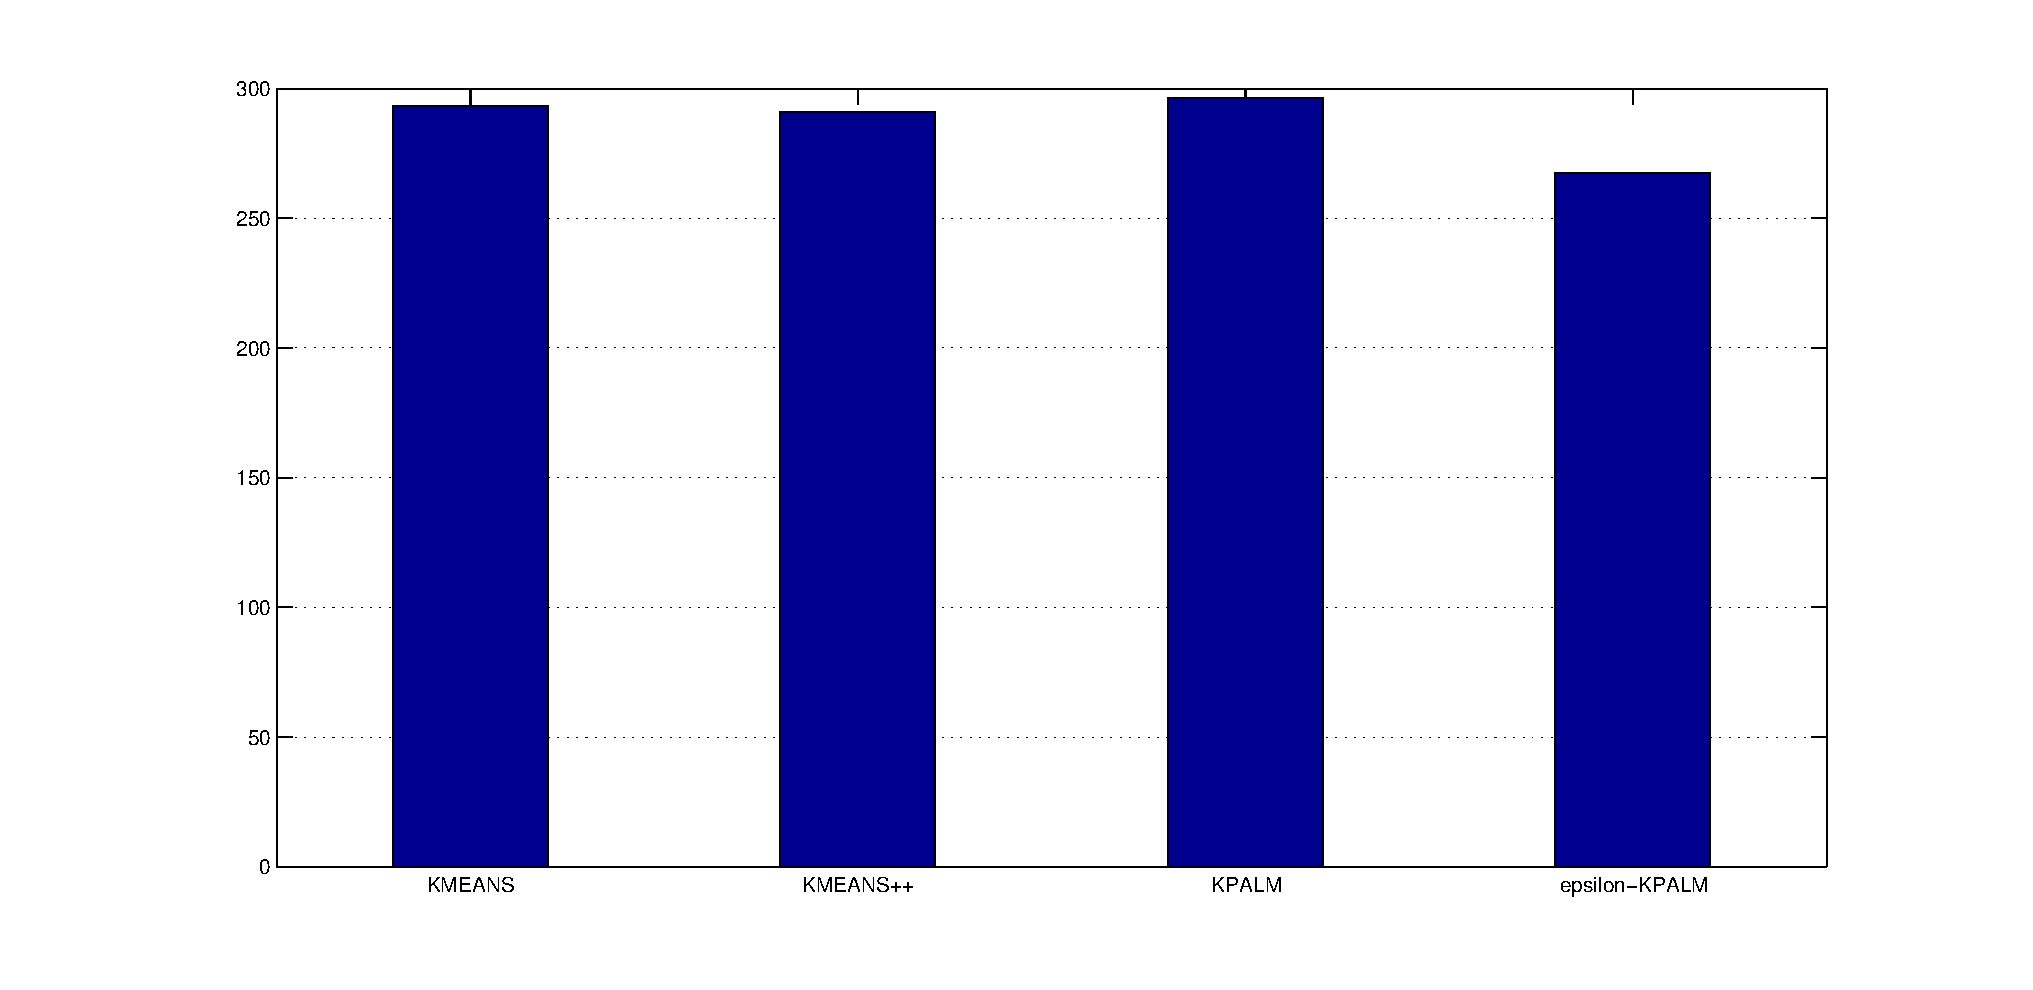
\includegraphics[width=\textwidth]{dense_gaussians_similarity}
        \caption{Dense Gaussians clustering.}
        \label{fig:dense_gaussians_similarity}
    \end{subfigure}
    \quad
    \begin{subfigure}[b]{0.8\textwidth}
        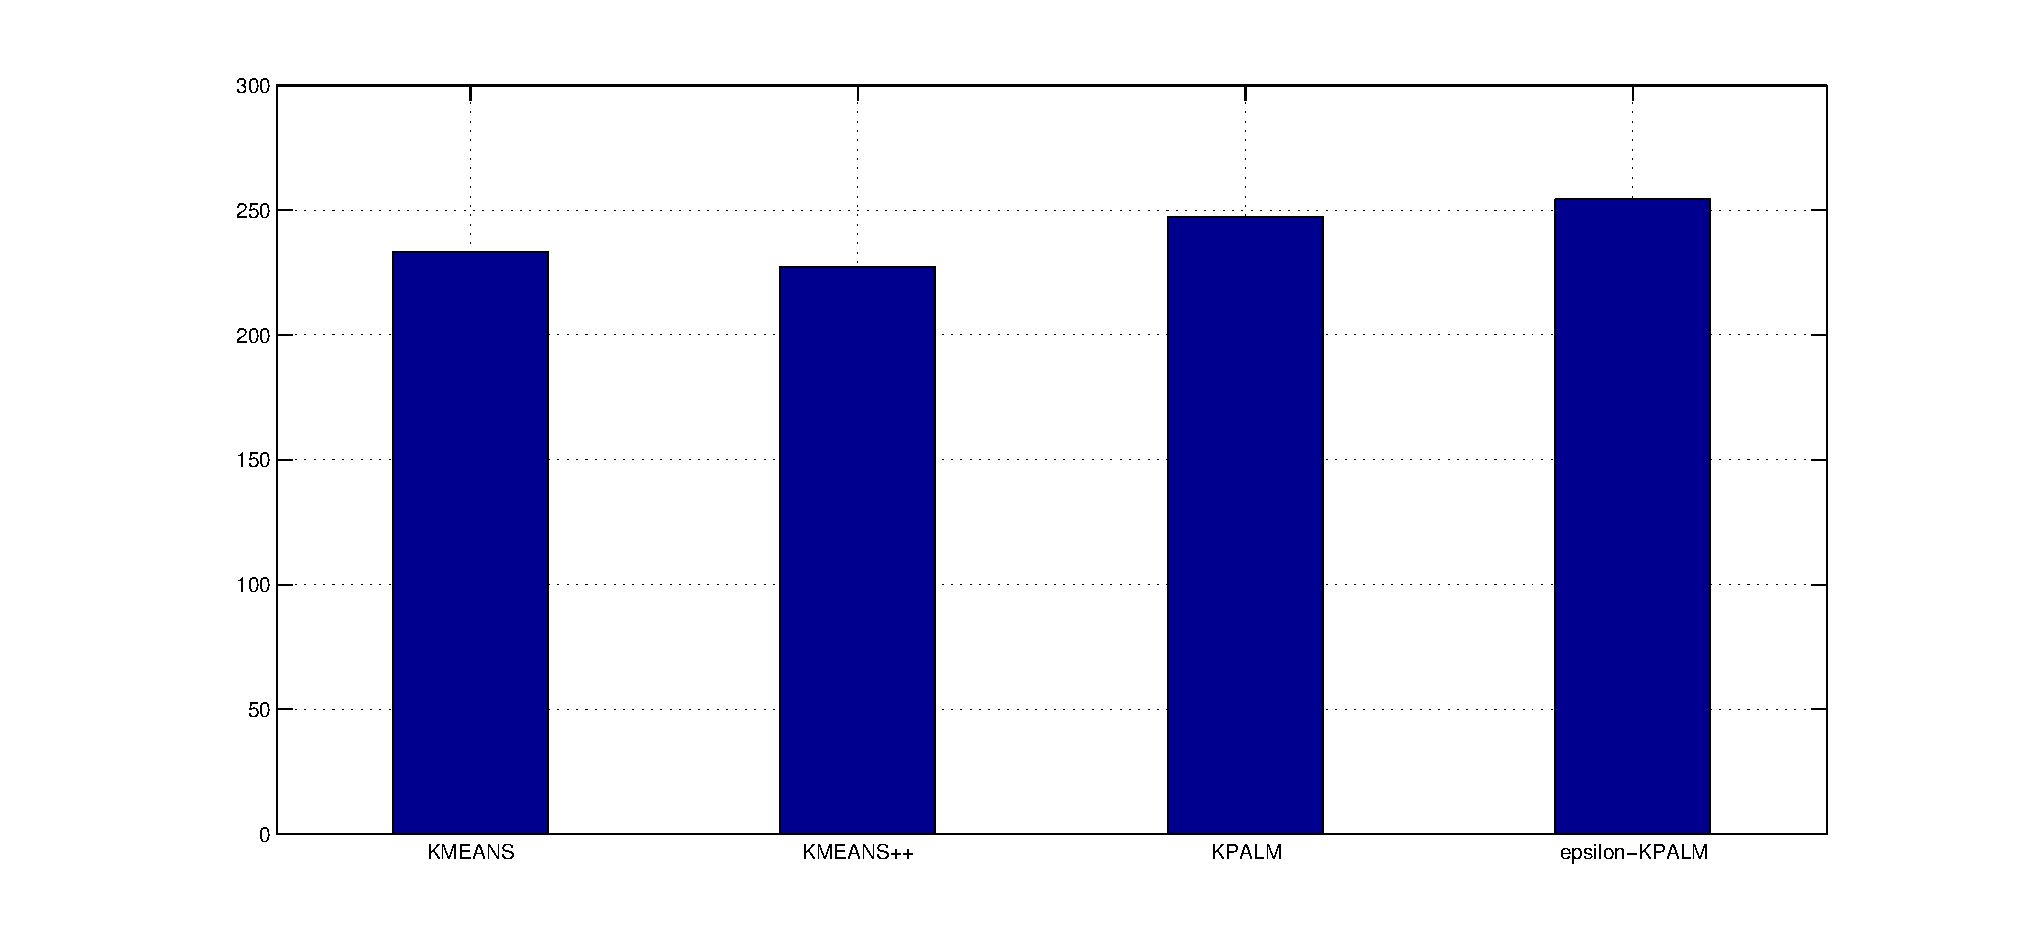
\includegraphics[width=\textwidth]{sparse_gaussians_similarity}
        \caption{Sparse Gaussians clustering.}
        \label{fig:sparse_gaussians_similarity}
    \end{subfigure}
    \caption{Results of clustering algorithms for dense and sparse datasets.}
    \label{fig:gaussians_similarity}
\end{figure}
\begin{figure}
    \centering
    \begin{subfigure}[b]{1\textwidth}
        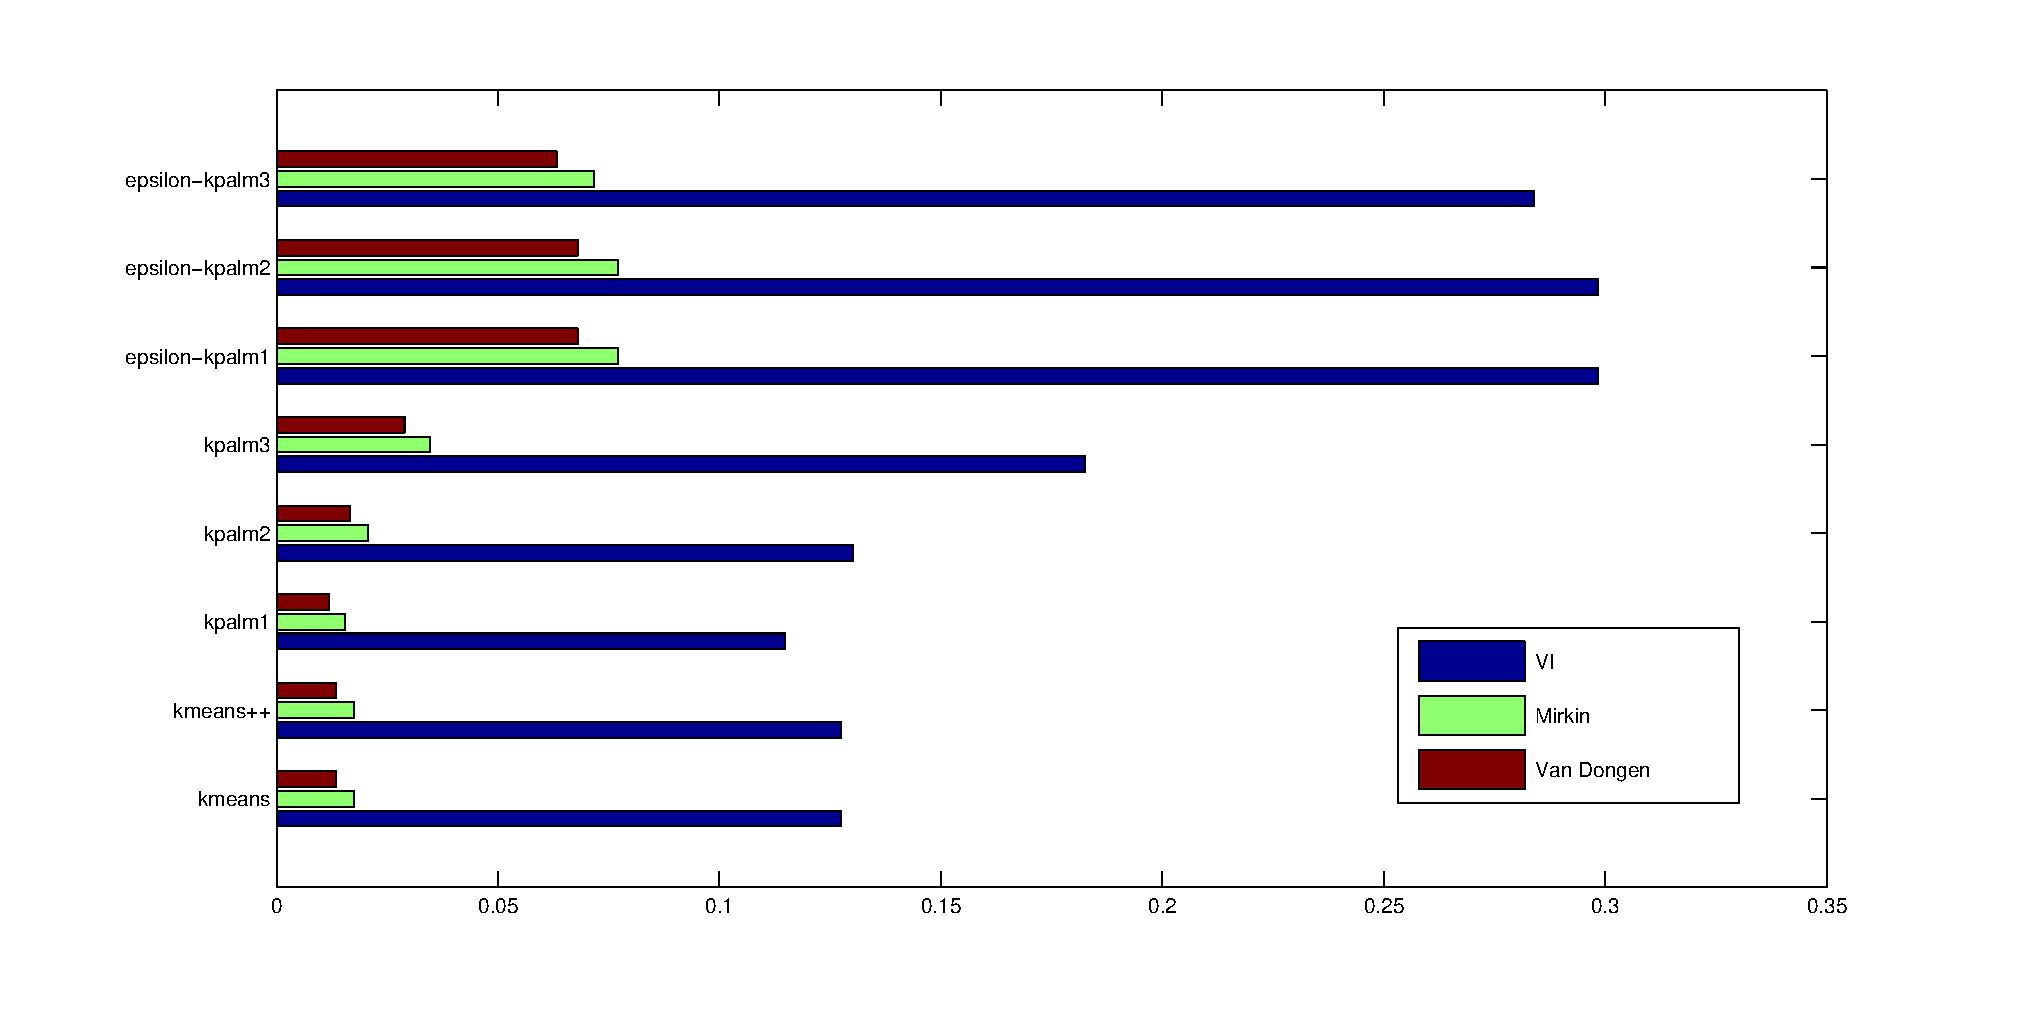
\includegraphics[width=\textwidth]{dense_gaussians_metrics2}
        \caption{Dense Gaussians metrics comparison.}
        \label{fig:dense_gaussians_metrics}
    \end{subfigure}
    \quad
    \begin{subfigure}[b]{1\textwidth}
        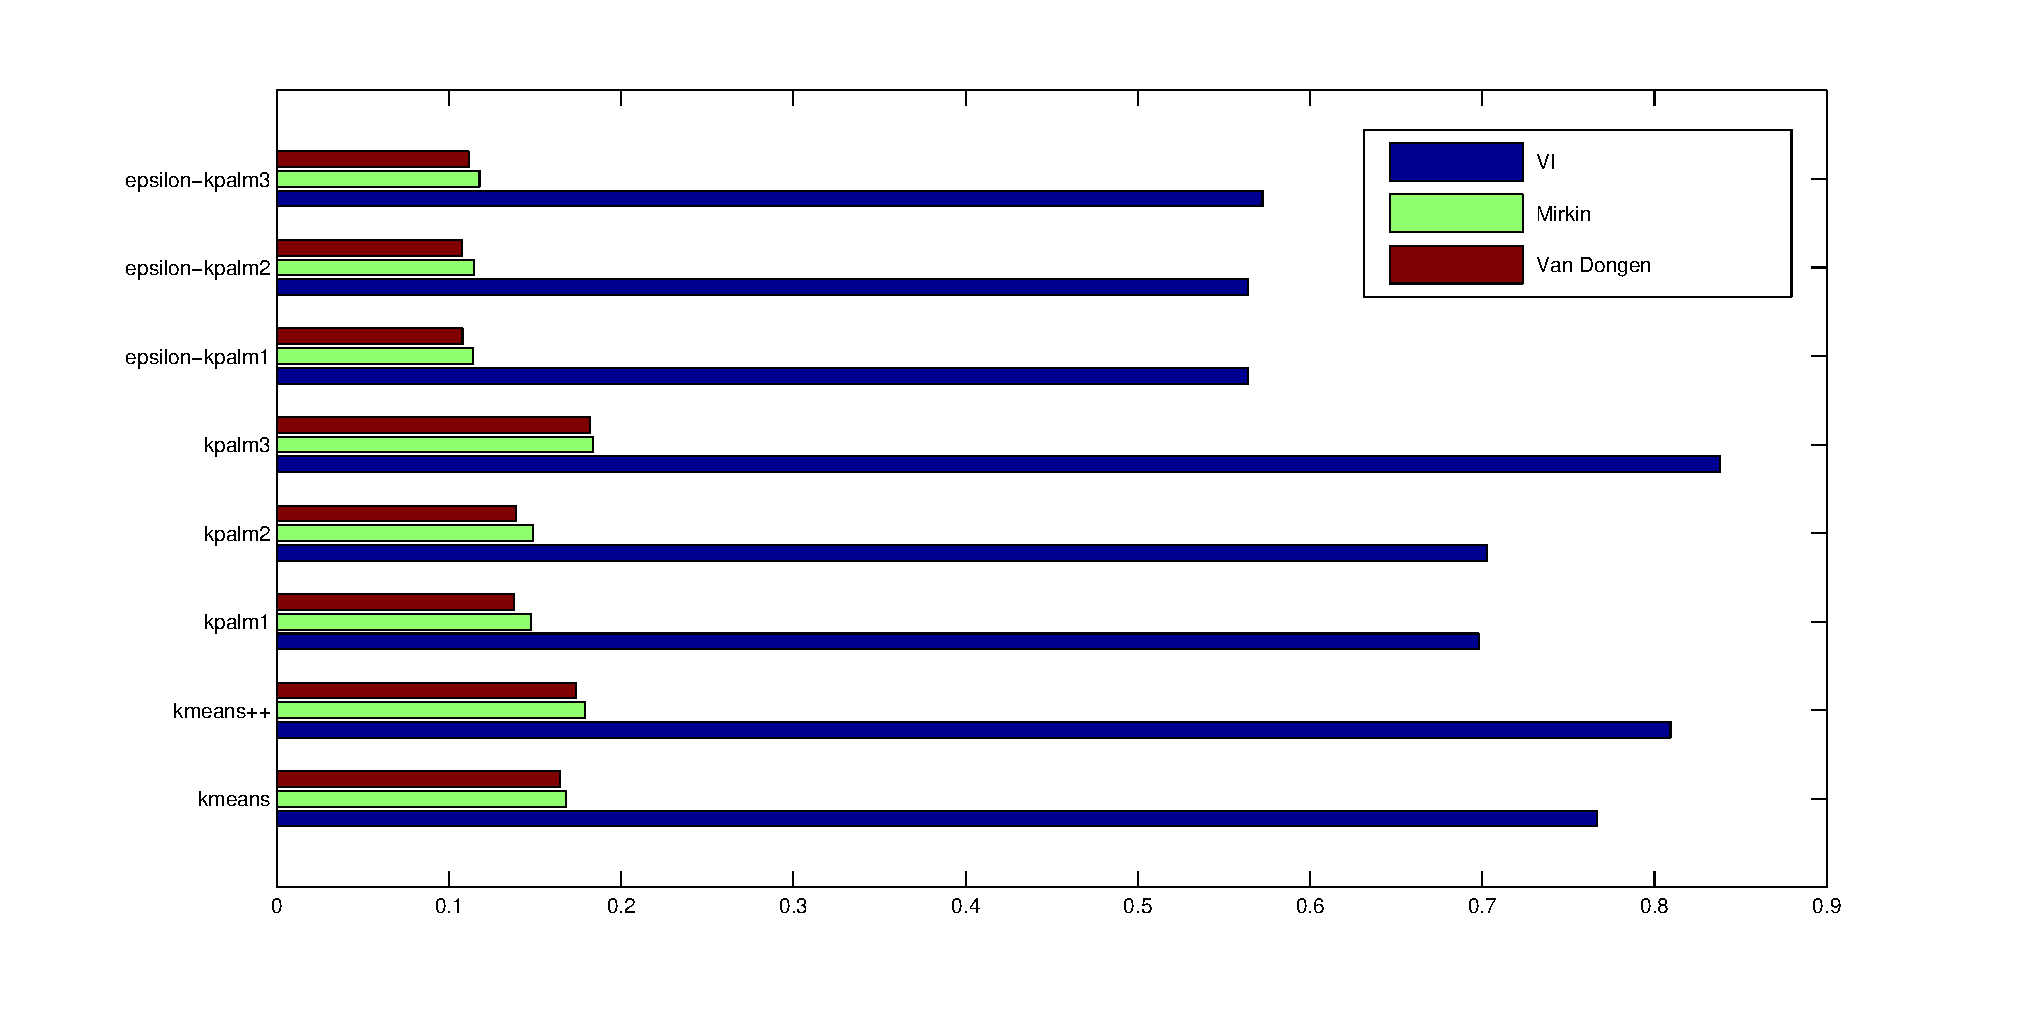
\includegraphics[width=\textwidth]{sparse_gaussians_metrics2}
        \caption{Sparse Gaussians metrics comparison.}
        \label{fig:sparse_gaussians_metrics}
    \end{subfigure}
    \caption{Comparison of metrics between clusterings for dense and sparse datasets.}
    \label{fig:gaussians_metrics}
\end{figure}
\clearpage
\section{Summary of Numerical Results}

From the conducted numerical experiments we deduce the following:
\begin{itemize}
	\item In the squared Euclidean setting, KPALM achieves lower objective function values than k-means. When using a more sophisticated initialization step, such as the one in k-means++, then k-means++ and KPALM++ achieve similar objective function values.
	\item k-means needs less number of iterations then KPALM to reach a certain precision.
	\item It is preferable to use dynamic update of $\alpha(t)$ parameter to achieve a faster convergence, both in KPALM and $\epsilon$-KPALM. Example for suitable choices can be $\alpha(t)= diam(\mathcal{A})/t$ and $\alpha(t)= diam(\mathcal{A})/2^t$.
	\item When the convex hulls of the desired clusters are mutually exclusive, algorithms which solve the clustering problem with the squared Euclidean distance are preferable to $\varepsilon$-KPALM. 
	This can be witnessed from the dense Gaussians example in \Cref{fig:gaussians}(\ref{fig:dense_gaussians}), and the comparison made in \Cref{fig:gaussians_metrics}(\ref{fig:dense_gaussians_metrics}), which shows that clusterings obtained with squared Euclidean algorithm are more similar to the desired clustering, and have lower distance in terms of clustering metrics, then the clustering obtained with $\varepsilon$-KPALM.
	\item In datasets with outliers, the clustering obtained with $\varepsilon$-KPALM is more similar to the desired clustering, in terms of clustering metrics, than the clusterings obtained via the squared Euclidean algorithms. This is witnessed from the sparse Gaussians example in \Cref{fig:gaussians}(\ref{fig:sparse_gaussians}), and the comparison made in \Cref{fig:gaussians_metrics}(\ref{fig:sparse_gaussians_metrics}). 
	Therefore, as expected, for data  with outliers, the choice of a norm instead of the squared norm is a more natural choice, and the $\varepsilon$-KPALM algorithm appears to be a promising algorithm to handle such data.
\end{itemize}